\documentclass{beamer} 
\usetheme{metropolis}
% \usecolortheme{spruce}
\setlength{\parindent}{0cm}
\usepackage{color}
\usepackage[utf8]{inputenc}
\usepackage[spanish]{babel}
\usepackage{amsmath}
\usepackage{amsfonts}
\usepackage{amssymb}
\usepackage{graphicx}
\usepackage{ragged2e}
\usepackage{caption}
\usepackage{subcaption}
\usepackage{tikz}
\usepackage{float}
\usepackage[skins,theorems]{tcolorbox}
\tcbset{highlight math style={enhanced,
  colframe=red,colback=white,arc=0pt,boxrule=1pt}}

\newtcolorbox{informacion}[2][]
{
  breakable,
  colframe = blue!5!white,
  colback  = blue!5!white,
  coltitle = blue!80!black,
  title    = \faInfo \hspace{5 mm} #2,
}


\title{
{\Large Mecánica de Materiales} \\
{\large II. Torsión}
}
\author{Pedro Jorge De Los Santos}
\institute{
    {\bf 
    Instituto Tecnológico de Celaya \\
    Departamento de Ingeniería Mecánica \\
    }
}

\apptocmd{\frame}{}{\justifying}{}
\begin{document}

\begin{frame}
\titlepage
\end{frame}

% Sección introducción
\section{Introducción}

\begin{frame}
\justifying
\frametitle{Torsión}

\begin{center}
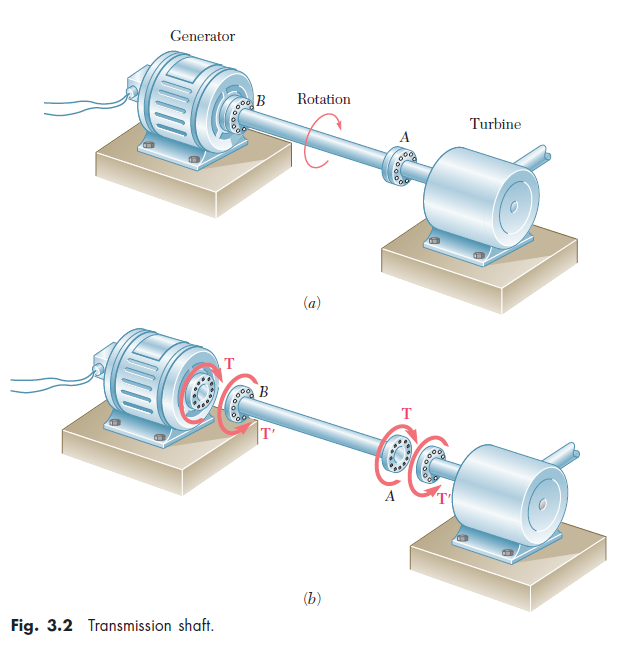
\includegraphics[width=0.6\textwidth]{img/flecha_transmision.PNG}
\end{center}

\end{frame}


\begin{frame}
\justifying
\frametitle{Análisis preliminar de esfuerzos}

Consideremos un eje sometido a torsión. Efectuando un corte perpendicular:

\begin{center}
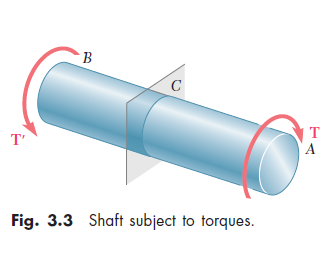
\includegraphics[width=0.55\textwidth]{img/shaft_torque.PNG}
\end{center}

\end{frame}


\begin{frame}
\justifying
\frametitle{Análisis preliminar de esfuerzos}

\begin{center}
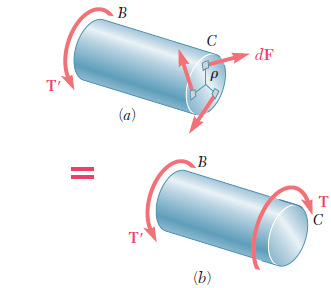
\includegraphics[width=0.35\textwidth]{img/shaft_torque_diagram.PNG}
\end{center}

$$ \int \rho \, dF = T $$

dado que $dF = \tau \, dA$, entonces:

$$ \int \rho \, (\tau \, dA) = T $$

\end{frame}


\begin{frame}
\justifying
\frametitle{Deformaciones en un eje circular}

\begin{center}
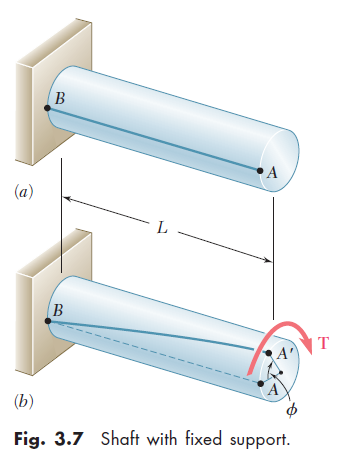
\includegraphics[width=0.35\textwidth]{img/shaft_fixed.PNG}
\end{center}

\begin{itemize}
\item $\phi$  - Ángulo de giro
\item $L$ - Longitud
\item $T$ - Par de torsión
\end{itemize}

% Necesitamos determinar una relación entre las tres variables anteriores.

\end{frame}


\begin{frame}
\justifying
\frametitle{Deformaciones en un eje circular}

\begin{center}
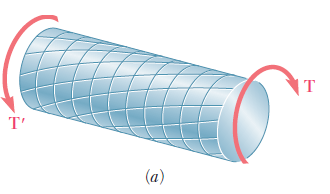
\includegraphics[width=0.45\textwidth]{img/shaft_deformations.PNG}
\end{center}

\begin{informacion}{Propiedades de ejes sometidos a torsión}
Cuando un eje circular se somete a torsión todas sus secciones transversales permanecen planas y 
sin distorsión.
\end{informacion}

\end{frame}


\begin{frame}
\justifying
\frametitle{Deformaciones en un eje circular}


\begin{minipage}{\linewidth}
  \centering
  \begin{minipage}{0.45\textwidth}
  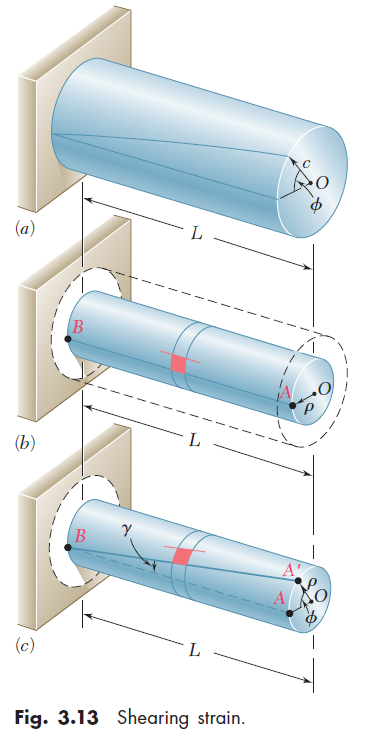
\includegraphics[width=0.85\textwidth]{img/shearing_strain.PNG}
  \end{minipage}
  \hspace{0.05\linewidth}
  \begin{minipage}{0.45\linewidth}
  Para valores pequeños de $\gamma$, puede expresarse la longitud de arco AA' como $AA' = L\gamma $, pero también 
  se tiene que $AA' = \rho \phi$, entonces, $L\gamma = \rho\phi$, o:

  $$ \gamma =\frac{\rho\phi}{L} $$
  \end{minipage}
\end{minipage}

\end{frame}


\begin{frame}
\justifying
\frametitle{Deformaciones en un eje circular}

La deformación a cortante es máxima en la superficie del eje, en donde $\rho = c$, entonces:

$$ \gamma_{max} = \frac{c\phi}{L} $$

Aplicando un poco de álgebra se tiene:

$$ \gamma = \frac{\rho}{c} \gamma_{max} $$

\end{frame}


\begin{frame}
\justifying
\frametitle{Esfuerzos en el rango elástico}

Ley de Hooke para esfuerzos a cortante:

$$\tau = G \gamma $$

Multiplicando la ecuación obtenida para $\gamma$ por G, se tiene:

$$ G\gamma = \frac{\rho}{c} G \gamma_{max} $$

$$ \tau = \frac{\rho}{c} \tau_{max} $$

\end{frame}


\begin{frame}
\justifying
\frametitle{Esfuerzos en el rango elástico}

\begin{center}
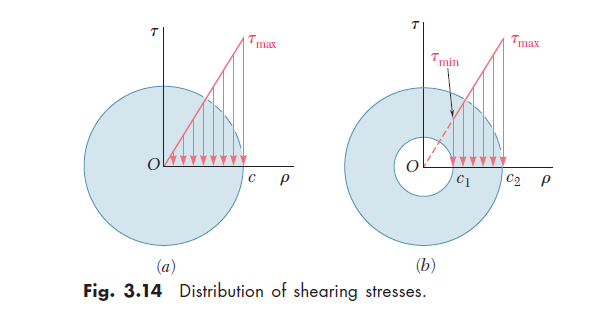
\includegraphics[width=0.75\textwidth]{img/stress_distribution.PNG}
\end{center}

$$ \tau_{min} = \frac{c_1}{c_2} \tau_{max} $$

\end{frame}


\begin{frame}
\justifying
\frametitle{Esfuerzos en el rango elástico}

De la formulación infinitésimal se tiene:

$$ T = \int \rho \tau \, dA = \frac{\tau_{max}}{c} \int \rho^2 \, dA $$

donde $\int \rho^2 \, dA = J$, siendo $J$ el momento polar de inercia respecto a $O$. Así:

$$ T = \frac{\tau_{max} J}{c}  \,\,\,\, \rightarrow \,\,\,\, \tau_{max} = \frac{Tc}{J} $$

Generalizando:

\begin{center}
\tcbhighmath{$$ \tau = \frac{T\rho}{J} $$}
\end{center}

\end{frame}



\begin{frame}
\justifying
\frametitle{Ángulo de giro en el rango elástico}

Igualando las siguientes ecuaciones:

$$ \gamma_{max} = \frac{c\phi}{L}  \,\,\,\,\,; \gamma_{max} = \tau_{max}/G $$

se puede obtener una expresión para el ángulo de giro:

\begin{center}
\tcbhighmath{$$ \phi =\frac{TL}{JG} $$}
\end{center}

Donde $\phi$ se expresa en radianes. La relación muestra que, dentro del rango elástico, el 
ángulo de giro $\phi$ es proporcional al par de torsión T aplicado al eje.
% \begin{center}
% 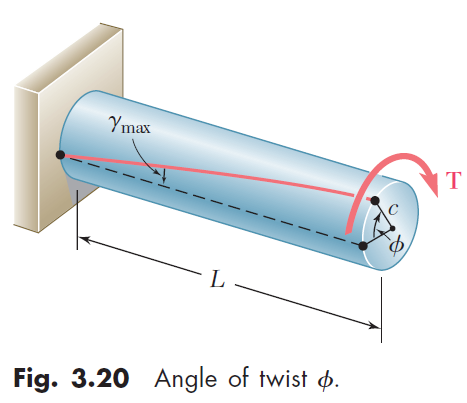
\includegraphics[width=0.45\textwidth]{img/angle_of_twist.PNG}
% \end{center}
\end{frame}


\begin{frame}
\justifying
\frametitle{Ángulo de giro en el rango elástico}

La fórmula anterior para el ángulo de giro puede utilizarse si el eje es homogéneo, si tiene una sección 
transversal uniforme y sólo si está cargado en sus extremos. Si el eje es sometido a par de torsión en 
lugares distintos a los extremos, o si consta de varias porciones con secciones transversales distintas y/o 
diversos materiales, debe dividirse en partes que satisfagan individualmente las condiciones 
requeridas por la ecuación establecida.
% \begin{center}
% \tcbhighmath{$$ \phi =\frac{TL}{JG} $$}
% \end{center}
\begin{center}
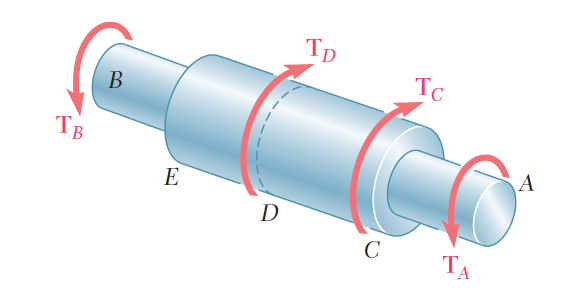
\includegraphics[width=0.45\textwidth]{img/multiple_section_shaft.PNG}
\end{center}
\end{frame}



\begin{frame}
\justifying
\frametitle{Ángulo de giro en el rango elástico}

El ángulo total de giro del eje, se obtiene sumando algebraicamente, los ángulos de giro de cada parte 
componente, expresándose como:

\begin{center}
\tcbhighmath{$$ \phi = \sum_i \frac{T_i L_i}{J_i G_i} $$}
\end{center}

El par de torsión interno $T_i$ en cualquier parte del eje se obtiene haciendo un corte a través de esa parte 
y dibujando el diagrama de cuerpo libre de la porción del eje situada a un lado de la sección.
\end{frame}



\begin{frame}
\justifying
\frametitle{Ángulo de giro en el rango elástico}

En el caso de un eje con sección circular variable, la ecuación del ángulo de giro puede aplicarse a un 
disco con grosor $dx$. Y el ángulo de giro total estaría dado por la integración de todos esos discos 
infinitésimales desde 0 a L, es decir:

\begin{center}
\tcbhighmath{$$ \phi = \int_0^L \frac{T\,\,dx}{JG} $$}
\end{center}

Donde, normalmente, J será una función dependiente de $x$, es decir $J(x)$.
\end{frame}



\begin{frame}
\justifying
\frametitle{Ejes de transmisión}

Las especificaciones principales que deben cumplirse en el diseño de un eje de transmisión 
son la potencia que debe transmitirse y la velocidad de rotación del eje.

\hfill \\

La potencia P asociada con la rotación de un cuerpo rígido sujeto a un par T es:

\begin{center}
\tcbhighmath{$$ P = T\omega $$}
\end{center}

Donde $\omega$ es la velocidad angular del cuerpo expresada en rad/s.
\end{frame}


\begin{frame}
\justifying
\frametitle{Ejes de transmisión}

Recuerde también que $\omega=2\pi f$, donde $f$ es la frecuencia de rotación, es decir, el 
número de revoluciones o ciclos por segundo. De lo cual se tiene:

\begin{center}
\tcbhighmath{$$ P = 2 \pi f T $$}
\end{center}

En el Sistema Internacional de Unidades la potencia se mide en watts (W), el torque en $N \cdot m$ y la frecuencia en Hz ($s^{-1}$)

\end{frame}



\begin{frame}
\frametitle{Referencias}

\begin{enumerate}
\item Beer, F. P. (2013). Mecánica de materiales. México, D.F: McGraw-Hill Interamericana.
\item Gere, J. M., Goodno, B. J., & León, C. J. (2014). Mecánica de materiales. Australia: Thomson Learning.
\item Gere, J., & Timoshenko, S. (1998). Mecánica de materiales. México, D.F: Thomson Learning.
\item Hibbeler, R. C., Murrieta, M. J. E., Molina, S. O., & Saldaña, S. S. (2011). Mecánica de materiales. Naucalpan de Juárez, México: Pearson educación.
\end{enumerate}
\end{frame}

\begin{frame}
\justifying
\frametitle{...}

El contenido de esta presentación está basado en las referencias bibliográficas básicas del curso. 
Si no se indica de manera explícita, las imágenes y diagramas corresponden a la referencia [1].

\end{frame}


\end{document}

